\section{Applications}
\label{sec:Applications}

The preceding sections organized self-improving agents by what is updated, namely model parameters or scaffolding, and by the signals that drive these updates. This section examines how these mechanisms appear across representative domains. Across applications, a common pattern is the use of sandboxed or otherwise controlled environments that provide feedback while limiting the cost of failure. \textbf{Software engineering} relies on compilers, tests, and continuous integration pipelines; \textbf{web automation} uses simulated or instrumented browsers; \textbf{games} provide resettable environments with explicit rules and outcomes; \textbf{scientific discovery} uses executable workflows, domain tools, and simulators; \textbf{embodied AI} relies on robotic simulators and limited real-world rollouts; and \textbf{general computer control} uses virtualized desktops or isolated operating-system environments. The fidelity, scalability, and cost of these environments shape each domain's dominant bottlenecks, improvement targets, and iteration modes, as summarized in Table~\ref{tab:applications_loops}.

\begin{figure*}[ht]
    \centering
    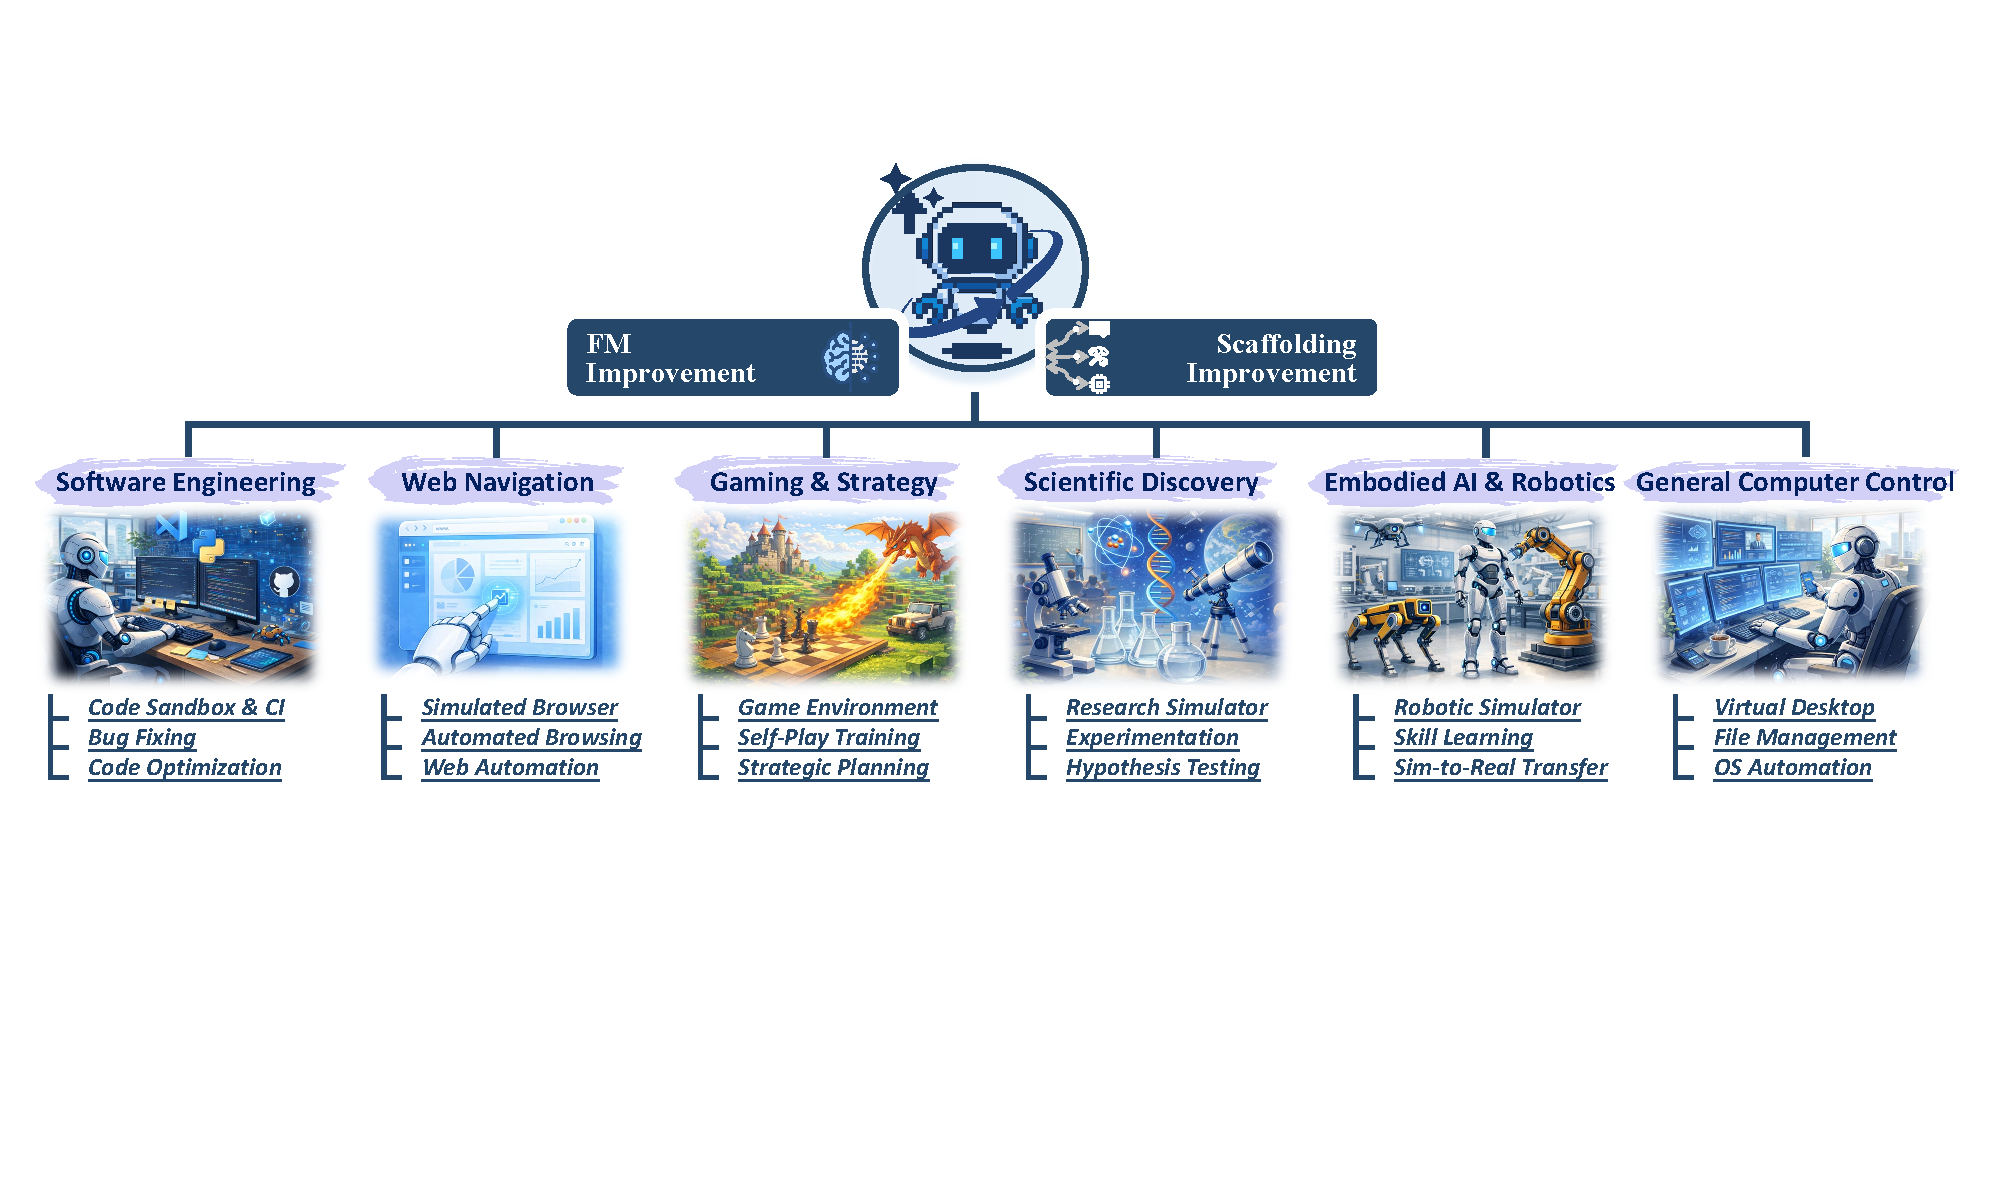
\includegraphics[width=1\linewidth]{fig/application.pdf}
    \caption{Representative application domains for self-improving agents.}
    \label{fig:application}
\end{figure*}

\subsection{Software Engineering}

Software engineering (SWE) is a useful testbed for self-improving agents because it provides dense and automatable feedback. Compilers, unit tests, linters, and continuous integration pipelines can turn many agent actions into checkable outcomes, making improvement easier to measure than in domains that rely on subjective evaluation. This property naturally supports both branches of our taxonomy: (i) \textbf{FM improvement}, where executable feedback is used to update model parameters $\theta$, and (ii) \textbf{scaffolding improvement}, where the model is fixed but the scaffold $\Sigma$ is revised. In SWE, the scaffold may include prompts, memory, tools, control logic, and, in some cases, the agent's own source code.


\paragraph{Evaluation substrate vs. self-improvement.}
It is important to distinguish evaluation environments from self-improving methods. SWE-bench provides a standardized suite of real GitHub issues, repositories, and test-based validation, enabling quantitative measurement of progress \citep{jimenez2024swebenchlanguagemodelsresolve}. Several related benchmarks have since been proposed \citep{deng2025swebenchproaiagents, aleithan2024swebenchenhancedcodingbenchmark, yang2025swebench}. However, systems such as SWE-agent \citep{yang2024sweagentagentcomputerinterfacesenable} and Agentless \citep{xia2024agentlessdemystifyingllmbasedsoftware} are better viewed as non-self-improving baselines under our definition. They may iterate within a task instance, but they do not, by default, perform persistent cross-interaction updates to $\theta$ or $\Sigma$. Their relevance here is methodological: they show that scaffold design can substantially affect performance, motivating the question of whether such scaffolds can be improved automatically rather than hand-engineered.

\paragraph{Scaffolding improvement via self-modifying software agents.}
A distinctive feature of SWE is that the agent itself is software, which makes direct scaffold or source-code modification feasible. The Darwin G"odel Machine operationalizes this idea by iteratively rewriting its own codebase and validating candidate modifications on coding benchmarks, producing a tree archive of improved descendants \citep{zhang2025darwingodelmachineopenended}. Building on this self-modification paradigm, the Huxley--G"odel Machine searches the space of self-modifications using an estimate of descendant performance, aiming to optimize long-term improvement potential rather than only immediate benchmark gains \citep{wang2025huxleygodelmachinehumanlevelcoding}.

Live-SWE-agent moves scaffold improvement from offline search to runtime self-evolution. Starting from a minimal scaffold, the agent edits and extends its own scaffold while solving real SWE tasks, so the current issue can inform future behavior \citep{xia2025livesweagentsoftwareengineeringagents}. SE-Agent studies a complementary trajectory-level mechanism, using cross-trajectory revision, recombination, and refinement to escape local optima in reasoning and action sequences \citep{lin2025seagentselfevolutiontrajectoryoptimization}. Viewed through $\Sigma=(p,m,T,g)$, these methods update increasingly rich scaffold components, from prompts and tool routines to full system code. They also highlight a SWE-specific lesson: performance depends not only on the base model, but also on the agent's executable interface to the codebase and its ability to preserve reusable problem-solving strategies across issues.

\paragraph{FM improvement from executable feedback.}
SWE also provides a direct route to FM improvement because test outcomes can serve as rewards or supervision. SWE-RL scales reinforcement learning to real-world software engineering tasks by using software-evolution data and executable signals to improve the underlying model \citep{wei2025swerladvancingllmreasoning}. Related work studies reinforcement learning in long-context and multi-turn SWE settings, with the goal of training models that can sustain extended tool-using interaction while remaining grounded in verification feedback \citep{golubev2025traininglongcontextmultiturnsoftware}. A practical limitation is that execution-based rewards can be sparse, noisy, or expensive, due to flaky tests, incomplete coverage, or costly environment setup. One complementary direction strengthens the executable signal itself by expanding the test suite: curiosity-driven planning can steer an LLM to generate tests that reach under-explored behaviors~\citep{amayuelas2026planning}. Execution-free feedback can therefore complement tests. SWE-RM explores reward-model-based scoring as a substitute for, or supplement to, unit tests, and analyzes which verifier properties transfer to reinforcement learning improvements \citep{shum2025swermexecutionfreefeedbacksoftware}.

\paragraph{Synthesis and open challenges.}
SWE exposes a useful contrast between the two improvement families. Scaffolding improvement is fast, modular, and model-agnostic, but it may overfit to benchmark tooling, repository conventions, or interaction protocols. FM improvement can internalize skills into $\theta$ and may transfer more broadly, but it is more expensive and more exposed to reward hacking and evaluation artifacts. Robust SWE self-improvement therefore requires (i) stronger evaluation against benchmark-specific search and verifier overfitting, such as benchmark mutation and stress testing, as well as (ii) hybrid loops in which scaffold-level discoveries are distilled into the base model only when they transfer beyond a fixed verifier or benchmark protocol \citep{garg2026savingswebenchbenchmarkmutation}.

\subsection{Web Navigation and Automation}

Web navigation and automation is a challenging domain for self-improving agents because the environment is dynamic, long-horizon, and often weakly verified. Web interfaces change frequently, the same user intent may be realized through different layouts or DOM structures, and failures often become visible only late in a trajectory. These properties make one-shot prompt engineering brittle and motivate improvement loops that persist across tasks. In our taxonomy, this domain supports both FM improvement, which updates $\theta$ from interaction data and feedback, and scaffolding improvement, which keeps $\theta$ fixed while updating $\Sigma$.

\paragraph{Evaluation and data substrate.}
A first line of work builds reproducible environments and demonstrations, which are prerequisites for systematic self-improvement. Mind2Web provides diverse instruction-following trajectories on real websites and supports supervised learning or imitation as an initial improvement step \citep{deng2023mindweb}. WebArena offers a self-hostable environment with long-horizon tasks and execution-based success criteria \citep{zhou2024webarena}. VisualWebArena extends evaluation to visually grounded web tasks and exposes failures in perception and grounding \citep{koh2024visualwebarenaevaluatingmultimodalagents}. WorkArena targets enterprise-style workflows and highlights the gap between current agents and routine knowledge-worker automation \citep{drouin2024workarenacapablewebagents}. BrowserGym further unifies evaluation across web-agent benchmarks, reducing experimental fragmentation and enabling more controlled comparisons of training and scaffold design \citep{workarena2024, chezelles2025browsergym}. These resources are not self-improving methods themselves, but they provide the data and measurement substrate needed to study improvement across interactions.

\paragraph{Scaffolding improvement with memory and grounding.}
In web environments, many improvements come from better scaffolding because robust grounding remains a central bottleneck. SeeAct couples visual understanding with action grounding on live websites, reducing brittle action selection in long-horizon execution \citep{zheng2024gptvision}. WebCoach is more directly aligned with self-improvement: it equips browsing agents with cross-session memory curated from new trajectories, allowing the agent to avoid repeated mistakes without retraining the base model \citep{liu2025webcoachselfevolvingwebagents}. ReAP similarly stores and reuses reflections over successful and failed trajectories to improve later web navigation \citep{azam2025reflectionbasedmemorywebnavigation}. These approaches instantiate scaffolding improvement by updating memory content, retrieval policies, and grounding-related structural artifacts that transfer across tasks.

\paragraph{FM improvement from interaction feedback.}
A complementary line updates $\theta$ using web interaction signals. \cite{patel2024largelanguagemodelsselfimprove} study self-improvement on WebArena by fine-tuning on mixtures of model-generated data and show that iterative training can improve web-agent capability. OpenWebVoyager proposes an exploration-and-feedback loop on real websites, improving its policy by learning from high-quality trajectories over multiple iterations \citep{he2024openwebvoyagerbuildingmultimodalweb}. Several works adopt reinforcement learning for long-horizon browser control. WebRL introduces a self-evolving online curriculum that generates new tasks from failures and combines it with outcome-supervised reward modeling \citep{qi2025webrl}. WebAgent-R1 trains web agents via end-to-end multi-turn reinforcement learning with binary success rewards and reports gains on WebArena-Lite \citep{wei2025webagentr1trainingwebagents}. Beyond navigation benchmarks, Agent Q studies learning from both successful and unsuccessful trajectories in WebShop and shows that such experience can improve generalization in multi-step web interaction \citep{putta2024agentqadvancedreasoning}. These FM-oriented methods also reveal a recurring difficulty: web feedback is often sparse, so improvement depends heavily on reward modeling, curriculum design, and the stability of the evaluation environment.

\paragraph{Synthesis and open challenges.}
Web automation faces a core challenge of self-improvement. This challenge comes from non-stationarity and weak observability. Page layouts and interaction flows often change over time. These changes can quickly weaken gains that were measured on static snapshots. Scaffolding improvement can help systems update grounding, state abstraction, and recovery behavior more quickly. Yet it can also overfit to specific websites. It may also increase safety risks, such as prompt injection or unintended high-impact actions~\citep{chen2026much}. FM improvement can support more transferable navigation skills. However, it depends on stable training signals and careful treatment of stale data. Progress therefore requires drift-aware evaluations. It also requires sandboxed protocols that separate safe exploration from irreversible actions. Finally, it requires grounding-centered improvements that transfer across layouts, DOM structures, and interaction conventions. These improvements should avoid memorizing site-specific patterns.



\subsection{Games and Strategic Reasoning}

Games remain a central testbed for self-improving agents because they provide repeatable interaction, well-defined objectives, and scalable feedback \citep{stanic2023learning}. Even when state spaces are large and long-horizon planning is required, games offer closed training loops in which agents can generate experience through self-play \citep{silver2018general, silver2017masteringchessshogiselfplay, Schrittwieser_2020, openai2019dota2largescale}. This makes the domain a natural fit for our taxonomy. Many game agents improve by updating model or policy parameters $\theta$ through reinforcement learning, while others improve by evolving the scaffold $\Sigma$, such as curriculum logic, planning routines, or memory structures that store reusable skills and experience.

\paragraph{FM improvement through self-play and outcome feedback.}
Recent work extends self-play to foundation models by using strategic games as sources of interaction data and outcome-based learning signals. SPAG trains language models through a two-player adversarial game and improves the policy via self-play reinforcement learning \citep{cheng2025selfplayingadversariallanguagegame}. SPIRAL studies multi-turn zero-sum self-play and shows that self-generated competitive interactions can provide a scalable signal for improving reasoning without human-labeled data \citep{liu2025spiralselfplayzerosumgames}. In adversarial game suites, SCO-PAL performs step-level policy optimization from game interaction data and identifies self-play as an effective opponent-selection strategy for strategic reasoning \citep{zhang2025enhancinglanguageagentstrategic}. Self-play reinforcement learning with limited initial data further examines how self-generated interactions can bootstrap improvement when external supervision is scarce \citep{fang2025serl}.

Imperfect-information and multi-agent settings introduce additional challenges in credit assignment and payoff estimation \citep{zhuge2023mindstorms, stanic2023learning}. MARSHAL proposes an end-to-end reinforcement learning framework for multi-agent self-play across cooperative and competitive strategic games, and reports transfer beyond games to multi-agent reasoning benchmarks \citep{yuan2026mars}. In negotiation-heavy environments, DipLLM studies fine-tuning for equilibrium-oriented policies in Diplomacy, providing a parameter-updating route for language-mediated strategic interaction \citep{xu2025dipllmfinetuningllmstrategic}. For high-variance payoff domains, SPRL uses reward shaping from self-play payoffs to stabilize training in complex strategic games \citep{anonymous2025llm}. Social deduction games provide another setting in which language agents can improve long-horizon strategic behavior through reinforcement learning from interaction outcomes \citep{xu2025languageagentsreinforcementlearning}.

\paragraph{Scaffolding improvement through curricula and reusable skills.}
Games also support scaffolding improvement because skills, procedures, and curricula can be represented explicitly and reused across interactions. Voyager exemplifies this paradigm in Minecraft by maintaining an expanding library of executable skills and an automatic curriculum that persists across tasks \citep{wang2023voyageropenendedembodiedagent}. Odyssey extends this direction with a structured open-world skill library and a planner--critic loop that improves long-horizon execution through skill reuse and prerequisite checking \citep{liu2025odysseyempoweringminecraftagents}.

Beyond open-world games, several methods construct reusable skills from interaction trajectories. Skill Set Optimization extracts high-reward subtrajectories, converts them into transferable skills, and prunes ineffective ones, yielding continual in-context policy improvement in game-like environments \citep{nottingham2024skillsetoptimizationreinforcing}. ExpeL shows that agents can accumulate experiences, distill them into natural-language lessons, and reuse them as in-context demonstrations for later decision making \citep{zhao2024expel}. In strategic and negotiation-heavy games, Richelieu maintains memory and reflection across self-play interactions, using accumulated experience to revise planning and negotiation behavior without weight updates at every step \citep{guan2024richelieu}. Recent self-evolving strategic systems similarly emphasize structural artifacts and long-term memory as the substrate for iterative strategy refinement across repeated games \citep{belle2025agentschangeselfevolvingllm}.


\paragraph{Synthesis and open challenges.}
Games offer unusually clear conditions for studying self-improvement. Their environments can be simulated, and feedback can be collected at scale. At the same time, games reveal risks that may be less visible in software engineering or web automation. Self-play can create brittle competence. A system may exploit a simulator or a narrow opponent distribution. It may then fail when the population shifts or when the rules change. In multi-agent games, improvement may also become non-monotonic. Strategic cycling can make progress difficult to measure. Evaluation against a fixed set of opponents may therefore give a misleading view of performance. Language-based strategy raises further safety concerns. These concerns include persuasion and deception. Win-loss objectives alone cannot govern such behaviors. Progress in this domain requires population-based evaluation that captures non-transitivity. It also requires training designs that promote robustness under rule and opponent shifts. Explicit constraints are also needed for language-mediated interaction.



% Domain icons (icon + tiny label)
\newcommand{\domSWE}{\faCode\;\textcolor{black!65}{{\scriptsize\textbf{SWE}}}}
\newcommand{\domWeb}{\faGlobe\;\textcolor{black!65}{{\scriptsize\textbf{Web}}}}
\newcommand{\domGame}{\faChessKnight\;\textcolor{black!65}{{\scriptsize\textbf{Game}}}}
\newcommand{\domSci}{\faFlask\;\textcolor{black!65}{{\scriptsize\textbf{Sci}}}}
\newcommand{\domRobot}{\faRobot\;\textcolor{black!65}{{\scriptsize\textbf{Emb}}}}
\newcommand{\domPC}{\faDesktop\;\textcolor{black!65}{{\scriptsize\textbf{PC}}}}

% Bullet marker
\newcommand{\bitem}{\textcolor{black!80}{\raisebox{0.15ex}{\scriptsize\textbullet}}\hspace{0.45em}}

% Wrapped cell: safe line breaks + vertical centering
\newcommand{\cellwrap}[1]{%
  \parbox[c]{\linewidth}{%
    \raggedright
    \setlength{\parskip}{0.15em}%
    \vspace{0.25em}%
    #1%
    \vspace{0.25em}%
  }%
}

% Bullet item (ends with \par so TeX can wrap nicely)
\newcommand{\bi}[1]{\bitem #1\par}

% Line item without bullet (for benchmarks column)
\newcommand{\li}[1]{#1\par}

% =========================================================
% Table (drop-in replacement)
% =========================================================
\begin{table*}[t]
\centering
\scriptsize
\setlength{\tabcolsep}{2.2pt}
\renewcommand{\arraystretch}{1.10}
\rowcolors{3}{gray!8}{white}

% Make X-columns behave like m-columns: vertical centering everywhere
\begingroup
\renewcommand{\tabularxcolumn}[1]{m{#1}}
\setlength{\emergencystretch}{1em}
\sloppy

\begin{tabularx}{\textwidth}{
>{\centering\arraybackslash}m{1.8cm}  % Domain
>{\raggedright\arraybackslash}X       % Sandbox / arena
>{\raggedright\arraybackslash}X       % Learning signal
>{\raggedright\arraybackslash}X       % Bottleneck
>{\raggedright\arraybackslash}X       % What improves most
>{\raggedright\arraybackslash}X       % Iteration mode
>{\raggedright\arraybackslash}X       % Benchmarks / representative systems
}
\toprule
\rowcolor{tab-blue}
\textcolor{white}{\textbf{Domain}} &
\textcolor{white}{\textbf{Sandbox and arena}} &
\textcolor{white}{\textbf{Learning signal}} &
\textcolor{white}{\textbf{Main bottleneck}} &
\textcolor{white}{\textbf{Primary improvement target}} &
\textcolor{white}{\textbf{Iteration mode}} &
\textcolor{white}{\textbf{Exemplars}} \\
\midrule

\domSWE &
\cellwrap{%
  \bi{Repository with compiler, unit tests, and CI}
  \bi{Failures are typically reversible}
} &
\cellwrap{%
  \bi{Deterministic binary outcomes (pass or fail)}
  \bi{Compilation errors}
  \bi{Static analysis signals}
} &
\cellwrap{%
  \bi{Patch correctness under repository constraints}
  \bi{Tool and interface efficiency}
} &
\cellwrap{%
  \bi{Mainly scaffolding}
  \bi{Some systems also self-edit code or fine-tune models}
} &
\cellwrap{%
  \bi{Online debugging per issue}
  \bi{Offline aggregation across issues}
} &
\cellwrap{%
  \li{\textbf{\hyperlink{cite.zhang2025darwingodelmachineopenended}{\makecell[l]{DGM(2025)}}}}
  \li{\textbf{\hyperlink{cite.wang2025huxleygodelmachinehumanlevelcoding}{\makecell[l]{HGM(2025)}}}}
  \li{\textbf{\hyperlink{cite.xia2025livesweagentsoftwareengineeringagents}{\makecell[l]{Live-SWE-agent\\(2025)}}}}
  \li{\textbf{\hyperlink{cite.zhang2026agentdevelreframingselfevolvingllm}{\makecell[l]{AgentDevel\\(2026)}}}}
} \\

\domWeb &
\cellwrap{%
  \bi{Simulated and standardized browsers}
  \bi{Partial observability of user interfaces}
} &
\cellwrap{%
  \bi{Sparse task completion signals}
  \bi{Long-horizon failures}
  \bi{Partial checks and heuristics}
} &
\cellwrap{%
  \bi{Grounding actions to dynamic layouts}
  \bi{Distribution shift over sites and pages}
} &
\cellwrap{%
  \bi{Scaffolding, including perception--action grounding, planning, and iterative repair}
  \bi{Trajectory and trace curation}
} &
\cellwrap{%
  \bi{Imitation style learning}
  \bi{Online correction along trajectories}
} &
\cellwrap{%
  \li{\textbf{\hyperlink{cite.qi2025webrl}{\makecell[l]{WebRL(2025)}}}}
  \li{\textbf{\hyperlink{cite.fang2025webevolver}{\makecell[l]{WebEvolver\\(2025)}}}}
  \li{\textbf{\hyperlink{cite.zheng2025skillweaverwebagentsselfimprove}{\makecell[l]{SkillWeaver\\(2025)}}}}
  \li{\textbf{\hyperlink{cite.zhang2026webrollbackenhancingwebagents}{\makecell[l]{WebRollback\\(2026)}}}}
} \\

\domGame &
\cellwrap{%
  \bi{Game engines with reliable reset}
  \bi{Self-play interactions}
} &
\cellwrap{%
  \bi{Win or loss outcomes, or scalar rewards}
  \bi{Clear terminal signals}
} &
\cellwrap{%
  \bi{Long-horizon planning}
  \bi{Imperfect information in some settings}
  \bi{Multi-agent non-transitivity}
} &
\cellwrap{%
  \bi{Model and policy parameters}
  \bi{Search and planning components}
} &
\cellwrap{%
  \bi{Self-play}
  \bi{Iterative policy improvement}
} &
\cellwrap{%
  \li{\textbf{\hyperlink{cite.guan2024richelieu}{\makecell[l]{Richelieu(2024)}}}}
  \li{\textbf{\hyperlink{cite.xu2025dipllmfinetuningllmstrategic}{\makecell[l]{DipLLM(2025)}}}}
  \li{\textbf{\hyperlink{cite.yuan2026mars}{\makecell[l]{MARSHAL\\(2025)}}}}
  \li{\textbf{\hyperlink{cite.cheng2025selfplayingadversariallanguagegame}{\makecell[l]{SPAG(2025)}}}}
} \\

\domSci &
\cellwrap{%
  \bi{Tool augmented research loops}
  \bi{Variable-cost evaluation}
} &
\cellwrap{%
  \bi{Experimental metrics}
  \bi{Tool outputs}
  \bi{Critique-based refinement}
} &
\cellwrap{%
  \bi{Expensive and noisy evaluation}
  \bi{Knowledge fragmentation}
  \bi{Heterogeneous tools and interfaces}
} &
\cellwrap{%
  \bi{Scaffolding, including tool orchestration, planning, and verification}
  \bi{Domain specialization}
} &
\cellwrap{%
  \bi{Propose, run, critique, and revise cycles}
  \bi{Mixed online and offline iteration}
} &
\cellwrap{%
  \li{\textbf{\hyperlink{cite.lu2024aiscientistfullyautomated}{\makecell[l]{The AI Scientist\\(2024)}}}}
  \li{\textbf{\hyperlink{cite.yamada2025aiscientistv2workshoplevelautomated}{\makecell[l]{AI-Scientist-v2\\(2025)}}}}
  \li{\textbf{\hyperlink{cite.ghafarollahi2024sciagentsautomatingscientificdiscovery}{\makecell[l]{SciAgents(2024)}}}}
  \li{\textbf{\hyperlink{cite.gottweis2025aicoscientist}{\makecell[l]{AI co-scientist\\(2025)}}}}
} \\

\domRobot &
\cellwrap{%
  \bi{Simulators with limited real-world rollouts}
  \bi{Safety constraints}
} &
\cellwrap{%
  \bi{Rewards and success signals}
  \bi{Real-world data is costly}
} &
\cellwrap{%
  \bi{Data collection and safety}
  \bi{Sim-to-real transfer}
  \bi{Dynamics credit assignment}
} &
\cellwrap{%
  \bi{Policy and model parameters via a data flywheel}
  \bi{Curricula and safety scaffolds}
} &
\cellwrap{%
  \bi{Collect data, retrain, and redeploy}
} &
\cellwrap{%
  \li{\textbf{\hyperlink{cite.bousmalis2023robocatselfimprovinggeneralistagent}{\makecell[l]{RoboCat(2023)}}}}
  \li{\textbf{\hyperlink{cite.zhou2024autonomousimprovementinstructionfollowing}{\makecell[l]{SOAR(2024)}}}}
  \li{\textbf{\hyperlink{cite.xu2024sinvigselfevolvinginteractivevisual}{\makecell[l]{SInViG(2024)}}}}
  \li{\textbf{\hyperlink{cite.yuan2025remacselfreflectiveselfevolvingmultiagent}{\makecell[l]{REMAC(2025)}}}}
  \li{\textbf{\hyperlink{cite.tian2025seear1treestructuredreinforcementfinetuning}{\makecell[l]{SEEA-R1(2025)}}}}  
} \\

\domPC &
\cellwrap{%
  \bi{Virtualized desktops}
  \bi{Standardized operating system tasks}
  \bi{Brittle user interfaces}
} &
\cellwrap{%
  \bi{Task completion and state checks}
  \bi{Long-horizon objectives}
} &
\cellwrap{%
  \bi{Diversity of applications}
  \bi{State tracking}
  \bi{Robust exploration of unseen apps}
} &
\cellwrap{%
  \bi{Scaffolding, including hierarchical planning, retrieval, and curricula}
  \bi{Action-trace training}
} &
\cellwrap{%
  \bi{Experience reuse and curriculum learning}
  \bi{Iterative trace collection}
} &
\cellwrap{%
  \li{\textbf{\hyperlink{cite.wu2024oscopilotgeneralistcomputeragents}{\makecell[l]{OS-Copilot\\(2024)}}}}
  \li{\textbf{\hyperlink{cite.xiao2025uigenie}{\makecell[l]{UI-Genie(2025)}}}}
  \li{\textbf{\hyperlink{cite.wu2025guireflectionempoweringmultimodalgui}{\makecell[l]{GUI-Reflection\\(2025)}}}}
  \li{\textbf{\hyperlink{cite.cheng2026evolvingtasksempoweringmultimodality}{\makecell[l]{SEA(2026)}}}}
} \\

\bottomrule
\end{tabularx}

\endgroup

\caption{Application arenas viewed as self-improvement loops.
Each domain induces a characteristic sandbox and learning signal, which shapes the dominant bottlenecks, the primary improvement target, and the iteration mode.}
\label{tab:applications_loops}
\end{table*}



\subsection{Scientific Discovery}

Scientific discovery has long motivated self-improving and curiosity-driven agents. Earlier work on artificial scientists and artificial curiosity framed learning agents as systems that invent informative experiments, reduce uncertainty, maximize learning progress or information gain, and iteratively improve their world models through self-generated interaction \citep{schmidhuber1990making, schmidhuber1991curious, storck1995reinforcement, schmidhuber1997s, schmidhuber2003exploring, schmidhuber2013powerplay, schmidhuber2015learning}. Contemporary FM-based scientific-discovery agents extend this line with large-scale language modeling, tool use, literature grounding, and automated workflow orchestration. In the FM era, the domain has become a high-impact setting for self-improving agents because it spans the full research lifecycle, including hypothesis generation, writing, experiment design, execution, analysis, and communication \citep{lu2024aiscientistfullyautomated, yamada2025aiscientistv2workshoplevelautomated, xiong2025beyond}.
Scientific discovery also differs from software engineering and web automation. Scientific environments are fragmented across subfields, rely on heterogeneous tools and data formats, and often provide feedback that is delayed, costly, or only partially automated. As a result, self-improvement in this domain is often realized as a research workflow that accumulates reusable artifacts across projects, rather than as a single response-level correction.

\paragraph{Evaluation substrate and feedback structure.}
Scientific discovery systems rely on diverse feedback signals. In computational research, agents can run code, simulations, and ablations. They can receive feedback from metrics, error traces, and experimental outcomes. In experimental science, feedback is often delayed and noisy. It is also constrained by reproducibility, cost, and safety. These properties shape which improvement pathway is feasible. FM improvement becomes more practical when reliable executable signals are available. Scaffolding improvement becomes more central when the main bottleneck lies in tool access, protocol selection, and evidence management across heterogeneous resources. More broadly, scientific discovery has long motivated intrinsic feedback criteria beyond immediate task success. These criteria include learning progress, information gain, compression progress, and informative experiment design \citep{storck1995reinforcement, schmidhuber2007simple, schmidhuber2010formal, schmidhuber2013powerplay}.


\paragraph{Scaffolding improvement through tool expansion and workflow evolution.}
A prominent trend frames self-improvement as a tool-augmented research loop. In this loop, the agent proposes hypotheses, invokes specialized tools, critiques results, and iterates. ChemCrow shows that language-model control over a broad set of chemistry tools can improve reliability and capability coverage. Under our definition, ChemCrow becomes self-improving when its tool repertoire or selection policy is updated across tasks \citep{m2024augmenting}. SciAgents emphasizes structured knowledge and multi-agent role specialization. It uses ontological graphs and in-situ learning to refine hypotheses across fragmented literature and data sources \citep{ghafarollahi2024sciagentsautomatingscientificdiscovery}. HoneyComb moves closer to explicit scaffold evolution. It constructs and refines domain tools and maintains a curated scientific knowledge base. These updates correspond to structural changes in the tool layer and retrieval policy \citep{zhang2024honeycomb}.


A second line focuses on end-to-end research orchestration. The AI Scientist and AI-Scientist-v2 implement iterative pipelines that generate ideas, write and debug code, run experiments, analyze results, and draft manuscripts, with repeated refinement driven by internal critique and experimental outcomes \citep{lu2024aiscientistfullyautomated, yamada2025aiscientistv2workshoplevelautomated}. AI co-scientist studies a complementary setting in which multi-agent debate and evolution are aligned with scientist-provided objectives and constraints; improvement appears as stronger hypothesis proposals under evidence tracking rather than as next-token likelihood optimization \citep{gottweis2025aicoscientist}. In our taxonomy, these systems primarily instantiate scaffolding improvement by revising planning strategies, experimental protocols, evaluation rubrics, and tool-use policies.

\paragraph{Model improvement through closed-loop experimentation.}
Parameter-level improvement is also possible in scientific discovery, though it often targets either scientific surrogate models or the agent policy itself. Self-driving laboratories and closed-loop experiment design provide a mature template: iterative experimentation updates internal models of the objective landscape, which then guide the next experiments \citep{tobias2025autonomous}. When reliable supervision is available, the agent policy can also be updated from experimental or computational outcomes. Coscientist integrates web search, code execution, and laboratory automation to design, plan, and run chemistry experiments \citep{boiko2023autonomous}. ORGANA and LLM-RDF further illustrate LLM-centered orchestration of experimental workflows and instrument-facing actions, opening a path toward learning from experimental success and failure when those signals can be formalized \citep{darvish2025organa, ruan2024automatic}. These directions are promising, but they also show that parameter-level improvement depends critically on feedback validity and on controls that prevent weak proxies or spurious correlations from being mistaken for scientific progress.

\paragraph{Synthesis and open challenges.}
Scientific discovery highlights three domain-specific challenges for self-improving agents. The first challenge is evaluation. Systems cannot easily verify novelty, correctness, or reproducibility on their own. Apparent improvements may instead reflect the exploitation of weak proxies. The second challenge is evidence management under heterogeneity. Improvements must persist across tools, data formats, and rapidly evolving literature. Stable scaffold evolution is therefore as important as policy learning. The third challenge is safety and governance. Experimental actions can be irreversible or hazardous. Scientific writing can also amplify misinformation when the evidence is weak. Progress in this domain therefore depends on reproducibility-centered evaluation, evidence tracking, and standardized experimental and computational protocols. It also depends on governance mechanisms that bound risk when agents propose or execute real-world scientific actions.



\subsection{Embodied AI and Robotics}

Embodied AI studies agents that perceive, reason, and act through a physical or simulated body. Compared with software engineering and web automation, this domain adds continuous state and action spaces, partial observability, safety-critical exploration, and the sim-to-real gap. These properties make self-improvement valuable but difficult. In practice, improvement is often realized as open-ended skill acquisition, where the agent accumulates reusable competence across tasks, embodiments, and environments.

\paragraph{Evaluation substrate and feedback structure.}
Embodied evaluation is typically conducted in simulation suites and real-robot trials, with feedback ranging from dense rewards to sparse success criteria and human interventions. Benchmarks such as RLBench, ManiSkill2, and Meta-World enable controlled comparison of improvement loops in simulation \citep{james2019rlbench, gu2023maniskill2unifiedbenchmarkgeneralizable, yu2020meta}. High-throughput simulators such as Isaac Gym reduce iteration cost and support large-scale training and ablations \citep{makoviychuk2021isaac}. Since evaluation protocols are discussed more generally in Section~\ref{sec:Evaluation}, we focus here on how embodied settings instantiate self-improvement mechanisms.

\paragraph{FM improvement through autonomous practice and data flywheels.}
A core route to embodied self-improvement is iterative data collection followed by policy updating, forming a data flywheel across interactions. RoboCat embodies this mechanism by training a multi-task, multi-embodiment manipulation policy and then using the trained policy to generate additional data for subsequent training iterations \citep{bousmalis2023robocatselfimprovinggeneralistagent}. MEDAL++ proposes a nearly autonomous reinforcement learning loop in which the robot learns to both perform and undo tasks, enabling reset-free practice and improving success rates with minimal human supervision \citep{sharma2023selfimprovingrobotsendtoendautonomous}. AutoRT scales real-world experience acquisition by using foundation models to propose diverse instructions and orchestrate robot fleets in the wild, producing large collections of interactions for later policy improvement \citep{ahn2024autortembodiedfoundationmodels}. Robot-Powered Data Flywheels formalize deployment as continual data collection and foundation-model adaptation, demonstrating improvement of vision-language components through robot-generated in-the-wild data \citep{grannen2025robotpowereddataflywheelsdeploying}. Self-Improving Embodied Foundation Models further propose a post-training recipe that uses shaped success detection to support autonomous robot practice and skill acquisition beyond imitation data \citep{ghasemipour2025selfimproving}.

\paragraph{Scaffolding improvement through curricula, memory, and safety logic.}
Embodied systems also benefit from scaffolding improvement because much of the difficulty lies in exploration, recovery, and safe interaction. RoboGen illustrates a generative simulation paradigm that automatically produces tasks, scenes, and supervision signals, effectively evolving the curriculum and data generation process across iterations \citep{wang2024robogenunleashinginfinitedata}. RACAS~\citep{ashley2026racas} accumulates the embodied knowledge of robot control through a structurally self-managed memory.
AutoRT can be viewed as a scaffold-level improvement approach when its instruction proposal policy, risk filters, and orchestration logic are iteratively refined to increase coverage while controlling safety violations \citep{ahn2024autortembodiedfoundationmodels}. Retrieval-driven upskilling and curriculum refinement provide another scaffold-level mechanism, allowing agents to accumulate reusable task recipes and training specifications across deployments \citep{zhu2025auraautonomousupskillingretrievalaugmented}. These structural artifacts can transfer across tasks even when the base model remains fixed.

\paragraph{Synthesis and open challenges.}
Embodied self-improvement faces multiple practical constraints, including safety, non-stationarity, and hardware cost. Real robots may experience sensor drift, rare but severe failures, and irreversible actions. These factors limit simple trial-and-error strategies. They also make the improvement process highly dependent on the design of safe exploration and recovery mechanisms. Simulators can support large-scale training. However, differences between simulation and reality often make improvements achieved in simulation difficult to transfer to real platforms. This gap calls for curriculum learning methods and data collection strategies that are specifically designed for transfer. Evaluation is also challenging. Some improvements may only reflect shortcuts found for specific benchmarks. Real deployment conditions also vary across laboratories and platforms. Progress in this field therefore depends on safety-aware improvement procedures, curriculum learning methods for sim-to-real transfer, and cross-embodiment evaluation practices. These practices are needed to distinguish genuine skill acquisition from overfitting to specific benchmarks.


\subsection{General Computer Control}

General computer control studies agents that operate full operating systems and third-party applications through graphical user interfaces. This setting is broader than web navigation because it requires control over files, windows, dialogs, shortcuts, and application-specific workflows, often across multiple applications within a single task. The main difficulty is environment diversity: the agent must adapt to unseen software and interface conventions. Self-improvement in this domain is therefore best understood as acquiring reusable procedures for learning new applications from interaction.

\paragraph{Evaluation substrate.}
Studying cross-interaction improvement requires reproducible operating-system environments with execution-based scoring. OSWorld provides a real computer environment that supports task setup and automated evaluation for open-ended computer tasks across operating systems \citep{xie2024osworldbenchmarkingmultimodalagents}. WindowsAgentArena offers a Windows-focused benchmark and scalable OS-level evaluation \citep{bonatti2024windowsagentarenaevaluating}. OSWorld-MCP extends evaluation beyond GUI actions by measuring tool invocation ability under the Model Context Protocol \citep{jia2025osworldmcpbenchmarkingmcptool}. Further discussion of evaluation appears in Section~\ref{sec:Evaluation}.

\paragraph{Scaffolding improvement via experience and procedural reuse.}
In general computer control, early gains often come from scaffold improvement because agents must handle long horizons and application-specific idiosyncrasies. Agent S introduces experience-augmented hierarchical planning with continual memory updates and retrieval over past trajectories. This enables cross-task gains through reusable procedural knowledge and supports transfer across OS benchmarks when memory and retrieval policies are maintained across interactions \citep{agashe2024agentsopenagentic}. SEAgent emphasizes autonomous mastery of novel software by generating curricula from simple to complex tasks and using a world-state model for step-wise trajectory assessment \citep{sun2025seagentselfevolvingcomputeruse}. These components instantiate scaffold evolution through task generation, evaluation heuristics, and reusable exploration routines that persist across episodes even when the base model is unchanged.

\paragraph{FM improvement through iterative training and verifier construction.}
A complementary line updates $\theta$ using automatically collected interaction traces and learned evaluative signals. UI-Genie proposes a self-improving pipeline that co-evolves an agent and a reward model for GUI tasks, addressing outcome verification and scalable data generation through reward-guided exploration \citep{xiao2025uigenie}. GUI-Reflection trains self-reflection and error correction abilities through iterative online reflection tuning, turning failures into supervision for subsequent parameter updates \citep{wu2025guireflectionempoweringmultimodalgui}. SEA proposes verifiable trajectory generation and step-wise reinforcement learning for long-horizon computer-use training \citep{cheng2026evolvingtasksempoweringmultimodality}. ComputerRL studies sustained end-to-end online reinforcement learning on OSWorld and introduces alternating training phases to mitigate optimization pathologies in extended RL \citep{lai2026computerrl}. PC Agent-E reduces reliance on large-scale human demonstrations by combining a small seed set with synthetic action decisions, providing an economical route to iterative policy improvement \citep{he2026efficient}.


\paragraph{Synthesis and open challenges.}
General computer control brings challenges that are not always apparent in purely web-based settings. Safety is a central concern because an agent may delete files, enter passwords, or initiate financial transactions. Any improvement process must therefore include safeguards and conservative recovery strategies. Verification is also difficult. In software engineering, unit tests can often provide clear feedback. In general computer control, success may depend on the operating system state, external accounts, or user-specific context. Another challenge is transfer. Agents need to learn new applications without relying too much on surface-level UI patterns. This calls for exploration strategies and curricula that encourage procedural abstractions. Progress will require reliable state-based verification where possible, cautious policies for irreversible actions, and adaptation mechanisms that support transfer across new applications. These issues also connect to early work on meta-reinforcement learning with self-modifying policies, where agents adapted by collecting long-term statistics about the effects of their own modifications during a lifelong trial \citep{Schmidhuber1994OnLH, schmidhuber1997shifting, schmidhuber1998reinforcement, schmidhuber1999general, schmidhuber2006goedelmachinesselfreferentialuniversal}.

